\subsection{Przetwarzanie i gromadzenie informacji w systemach rozproszonych, autonomicznych i sieciach IoT}

\begin{figure}[H]
	\centering
	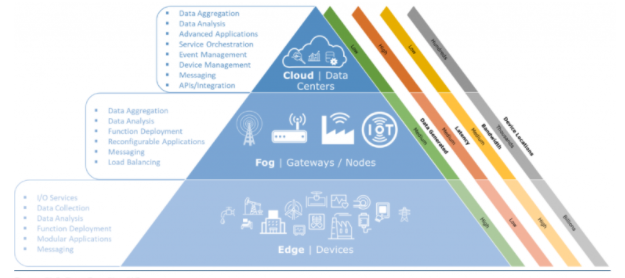
\includegraphics[width=0.3\linewidth]{S9.png}
\end{figure}

Architektury, warstwy” wykorzystywane w przetwarzaniu danych w takich systemach to:

\begin{itemize}
	\item \textbf{Cloud} (chmury obliczeniowe)
	\item \textbf{Fog} (mgła obliczeniowa)
	\item \textbf{Edge} (urządzenia brzegowe)
	\item \textbf{Mist} (sensor/ end-node)
\end{itemize}

\subsubsection{Cloud}

Zazwyczaj urządzenia IoT mają małą moc obliczeniową i niewielką ilość pamięci, z tego powodu rozwiązania chmurowe są bardzo popularne, ponieważ zapewniają skalowalne zasoby do przetwarzania i przechowywania danych na żądanie. Dane z sensorów są transportowane do centrum obliczeniowego, gdzie są przetwarzane, a wynik jest przesyłany do zasubskrybowanych aplikacji. Ponadto centra obliczeniowe mogą przechowywać dane w celu analizy i wydobycia z nich wiedzy. \\

Zalety chmury obliczeniowej to:

\begin{itemize}
	\item brak konieczności utrzymywania własnej infrastruktury obliczeniowej.
	\item możliwość szybkiej realizacji projektów i testowania koncepcji bez dużych zakupów IT i dużych kosztów początkowych (płaci się tylko za zużyte zasoby).
	\item jeżeli dane wysyłane/odczytywane są rzadko to wykorzystanie rozwiązań chmurowych jest tańsze, bo nie trzeba pozostawiać w stanie bezczynności dedykowanego sprzętu i oprogramowania.
	\item duża wydajność, elastyczność, skalowalność
	\item niezawodność przy założeniu stabilnego połączenia
	\item łatwość w wykorzystaniu tych samych danych przez wiele grup/aplikacji \\
\end{itemize}

Jednak ta technologia ma swoje wady np:

\begin{itemize}
	\item wymaga stałego dostępu do Internetu, często o dużej przepustowości
	\item niektóre przedsiębiorstwa mogą być niechętne umieszczaniu krytycznych danych w chmurze z powodu obawy o bezpieczeństwo danych
	\item nie nadaje się do aplikacji, które potrzebują danych do analizy w czasie rzeczywistym, ponieważ trzeba wysłać dane z węzła aż do chmury co generuje opóźnienia \\
\end{itemize}

\subsubsection{Fog}

W mgle obliczeniowej przetwarzanie danych odbywa się na urządzeniach, które znajdują się na krawędzi sieci. Do urządzeń brzegowych należą routery, switche, access pointy wifi,  set-top-boksy, stacje bazowe itd. Urządzenia te nie są już używane wyłącznie do przesyłania danych, lecz posiadają znaczne możliwości obliczeniowe oraz pamięć masową. \\

Zadania obliczeniowe, które w przeciwnym razie musiałby zostać przesłane do jakiejś chmury mogą zostać zrealizowane lokalnie, minimalizuje to czas przetwarzania, a co jest szczególnie ważne dla aplikacji, które muszą działać w czasie rzeczywistym. \\

Architektura mgły obliczeniowa może być scentralizowana lub rozproszona lub być kombinacją obu. W architekturze scentralizowanej każdy węzeł działa pod węzłem centralnym, zarządzanie taką siecią jest łatwe, ale gdy liczba podłączonych urządzeń wzrasta to staje się to wyzwaniem. W rozproszonej architekturze urządzenia współdziałają w sposób peer-to-peer.. Obciążenia obliczeniowe są rozproszone pomiędzy urządzeniami,. Każdy z węzłów mgły komunikuje się z innymi np. w celu podziału pracy. \\

Można wyróżnić 3 rodzaje komunikacji:

\begin{itemize}
	\item \textbf{Machine-to-machine} - dane generowane przez jedno urząðzenie są konsumowane przez inne urządzenia
	\item \textbf{machine-to-people} - dane generowane przez urządzenia są konsumowane przez ludzi i i vice versa
	\item \textbf{people-to-people} - dane generowane przez ludzi są konsumowane przez ludzi \\
\end{itemize}

Czas trwania tych interakcji może wynosić od sekund do dni. Na przykład, interakcja w aplikacjach działających w czasie rzeczywistym trwa od kilku sekund do kilku minut. Natomiast analiza transakcyjna może trwać kilka dni. \\

Architektura Fog zmniejsza również obciążenie połączeń sieciowych, ponieważ większość komunikacji dzieje się w pobliżu użytkownika, więc bardzo niewiele łączy sieciowych jest zaangażowanych w dane/usługi we mgle mając na uwadze, że w przypadku architektury Cloud cała sieć może zaangażować się w świadczenie usługi do użytkownika końcowego. \\

Oprócz dostarczania usługi dla użytkowników końcowych może również zarządzać ruchem sieciowym, jak również w razie potrzeby może korzystać z zasobów chmury, gdy przetwarzanie danych przekracza jej możliwości. \\

Wady:

\begin{itemize}
	\item magazynowanie danych,urządzenia nie mają odpowiedniej pojemności. do przechowywania dużych ilości danych przez bardzo długi czas ze względu na różne ograniczenia fizyczne.
	\item architektura ze względu na ograniczoną moc obliczeniową urządzeń IoT, co sprawia, że mgła nie nadaje się do użytku dla usług związanych z ciężkimi obliczeniami. \\
\end{itemize}

Globalna koordynacja: Architektura chmury wspiera globalną koordynację, ponieważ jest to scentralizowana architektura, w której chmura może nawet koordynować pomiędzy różnymi urządzeniami Fog w całym obszarze globu

\subsubsection{Edge}

Edge computing może być używany do przetwarzania danych bezpośrednio na urządzeniach, które mają dołączone czujniki lub urządzeń bramowych, które są blisko czujników. W związku z tym, obliczenia krawędziowe mogą umożliwić urządzeniom przetwarzanie danych bez polegania na chmurze lub mgle. Przetwarzając dane bliżej krawędzi, obliczenia krawędziowe mogą umożliwić urządzeniom przetwarzanie danych w czasie zbliżonym do rzeczywistego. W związku z tym, obliczenia krawędziowe mogą zmniejszyć koszty ogólne w scentralizowanej chmurze. \\

Obliczenia krawędziowe mogą być wykorzystywane w podłączonych domach do wykonywania zadań, takich jak włączanie grzejnika lub oświetlenia w czasie zbliżonym do rzeczywistego.

\subsubsection{Mist}

Mist computing to ekstremalna wersja edge computingu, zwykle składa się z mikrokontrolerów i czujników. Umożliwienie zbierania danych poprzez zdolności obliczeniowe i komunikacyjne samego czujnika. \\

Obsługa komunikacji wymaga często większość mocy obliczeniowej mikrokontrolera, zbierając surowe dane i filtrując je jesteśmy w stanie wysyłać tylko istotne dane do stacji bazowej, routera czy też serwera, co umożliwia oszczędzanie energii i przepustowości. \\

Przetwarzanie danych na urządzeniu brzegowym obejmuje często takie rzeczy jak:

\begin{itemize}
	\item Normalizacja lub przekształcenie danych do jednolitego formatu, zapewniając, że format ten jest zgodny z aplikacją.
	\item Dane “opakowaniowe” w sposób, który jest bezpieczny i łączy dane w “praktyczną partię”.
	\item Walidacja danych w celu zapewnienia ich zgodności z szeregiem ustalonych reguł.
	\item Sortowanie danych w celu utworzenia preferowanej sekwencji
	\item “Podsumowywanie/kompresowanie danych” w celu zmniejszenia objętości i wyeliminowania niepotrzebnych lub niepożądanych szczegółów.
	\item Filtrowanie powtarzających się, nieaktualnych lub niepożądanych danych w celu zwiększenia ich dokładności.
	\item Wzbogacanie danych za pomocą dodatkowych powiązanych informacji (metadata)
\end{itemize}
